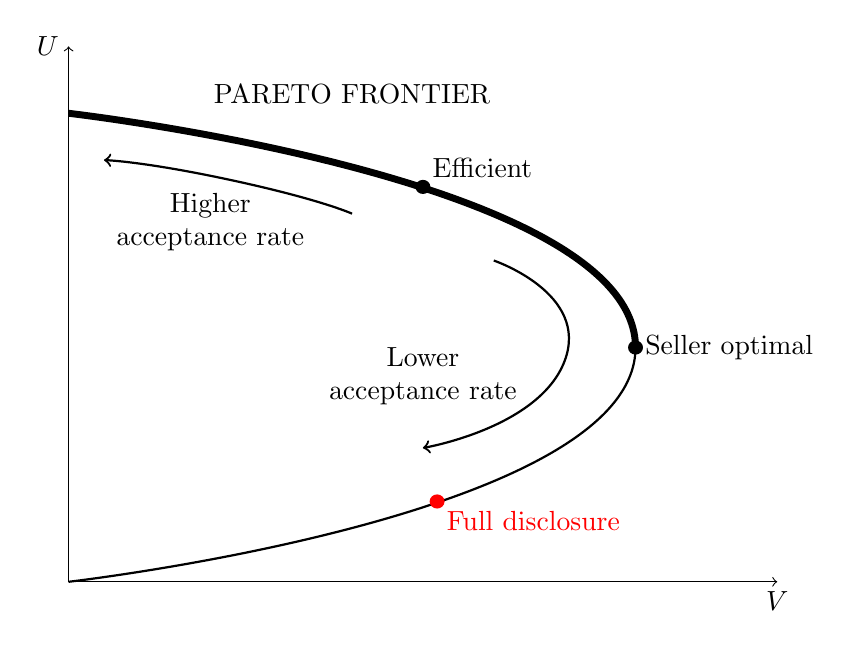
\begin{tikzpicture}[xscale=.9,yscale=.85] 

		\draw [<->] (0,8) node (yaxis)[left] {$U$} 
		        |- (10,0) node (xaxis) [below] {$V$};
	\def\mycoordinates{(0,0) (8,3.5) (0,7)}

	%\draw[step=1cm,gray,very thin] (0,0) grid (10,8);

	\def\mycoordinates{(0,0) (8,3.5) (0,7)}

	\draw[thick] plot [smooth,tension=1.3] coordinates {\mycoordinates};
	\begin{scope}
	    \clip (0,3.5) rectangle (10,8);
	    \draw [line width=2.5] plot [smooth,tension=1.3] coordinates {\mycoordinates};
	  \end{scope}

        %\fill (0,0)  circle (2pt) ;
	%\node at (.9,.2)[above] {$\bar\rho=0$};
      \fill (8,3.5)  circle (3pt) ;
	\node at (8,3.5)[right] {Seller optimal};
       % \fill (0,7)  circle (2pt) ;
	%\node at (0,7.5)[right] {$\bar\rho^{max}\leq 1$};
	\coordinate (E) at (5,5.9);
      \fill (E)  circle (3pt) ;
	\node at (E)[above right] {Efficient};
	

	%\draw[thick] plot [smooth,tension=1.3] coordinates {\mycoordinates};

%	\draw [->,thick] (4,5.5) to  (.5,6.3);
	\draw[thick,->] plot [smooth,tension=1.3] coordinates {(4,5.5)  (2.3,6) (.5,6.3)};

	\draw[thick,->] plot [smooth,tension=1.3] coordinates {(6,4.8) (7,3.3) (5,2)};

%	\draw [->,thick] (6,4.5) to  [out=-30,in=30] (5,2);


	\node at (4,7) [above] {PARETO FRONTIER};


	\node at (2,4.8) [above, align=center] {Higher\\acceptance rate};

	\node at (5,2.5) [above,align=center] {Lower\\acceptance rate};


	\coordinate (A) at (5.2,1.2);
        \fill[red] (A)  circle (3pt) ;
	\node at (A) [below right,red] {Full disclosure};




        
\end{tikzpicture}